\documentclass[11pt, a4paper]{article}

% --- Paquets essentiels ---
\usepackage[utf8]{inputenc}     % Encodage
\usepackage[T1]{fontenc}        % Fontes
\usepackage[french]{babel}      % Langue française
\usepackage{graphicx}
\usepackage{xcolor}             % Pour la couleur du code
\usepackage{minted}             % Le paquet magique pour le code
\usepackage[margin=2cm]{geometry}
\usepackage{titlesec}
\usepackage{float}
\usepackage{placeins}

\newcommand{\sectionbreak}{\clearpage}
\setlength{\fboxsep}{2pt} % Teste avec 0pt si tu ne veux absolument aucune marge

% --- Configuration esthétique ---
\definecolor{mycodeback}{rgb}{0.1,0.1,0.25} % Couleur de fond bleu
\setminted{
    fontsize=\footnotesize,  % Taille de la police
    linenos,
    bgcolor=mycodeback,
    style=native, % Style de couleur (ex: tango, monokai, colorful)
    breaklines=true,
    stripnl=true
}

\begin{document}

\begin{titlepage}

    \begin{flushleft}
        \large
        \textsc{BOUCHUT} Tanguy \\
        \textit{Grenoble INP - PHELMA}
    \end{flushleft}

    \vfill

    \begin{center}
        \Huge \textbf{RAPPORT ARCHITECTURE AVANCÉE} \\
        \vspace{1cm}
        \Large Conception d'un cœur RISCV
    \end{center}

    \vfill

\end{titlepage}

\tableofcontents % Génère le sommaire automatiquement

\section{Conception de l’architecture matérielle}

Tout d’abord, il a fallu implémenter tous les composants qui font partis du cœur RISCV. Nous les avons implémentés dans l’ordre dans lequel ils interviennent pendant un cycle d’horloge.

\subsection{FETCH}

\subsubsection{Le PC FETCH}

Tout d'abord nous avons commencés par le PC fetch qui détermine et fournit l'adresse de la prochaine instruction à exécuter.

\inputminted[
    firstline=24,
    lastline=43
]{vhdl}{../ENSSAT-RISCV-design-student/src/riscv/fetch/fetch.vhd}

\subsubsection{Le testbench du PC FETCH}

\inputminted[
    firstline=47,
    lastline=78
]{vhdl}{../ENSSAT-RISCV-design-student/src/riscv/fetch/fetch_tb.vhd}

\subsubsection{Program ROM} Ensuite, nous nous sommes concentrés sur le program ROM qui lit la mémoire et renvoie l'instruction correspondant à l'adresse demandée.

\inputminted[
    firstline=48,
    lastline=57
]{vhdl}{../ENSSAT-RISCV-design-student/src/riscv/rom/mem_rom.vhd}

\subsubsection{Le testbench du program ROM} Pour écrire le testbench du ROM, il a fallu faire plusieurs modifications au fichier original. Tout d'abord, il a fallu importer les fichiers de configuration.

\inputminted[
    firstline=9,
    lastline=10
]{vhdl}{../ENSSAT-RISCV-design-student/src/riscv/rom/mem_rom_tb.vhd}

Ensuite, il a fallu corriger les erreurs en remplaçant \verb|RAM_ADDR_BITS| par \verb|ROM_ADDR|.

\inputminted[
    firstline=23,
    lastline=23
]{vhdl}{../ENSSAT-RISCV-design-student/src/riscv/rom/mem_rom_tb.vhd}
\inputminted[
    firstline=30,
    lastline=30
]{vhdl}{../ENSSAT-RISCV-design-student/src/riscv/rom/mem_rom_tb.vhd}

Corriger le generic map.

\inputminted[
    firstline=39,
    lastline=42
]{vhdl}{../ENSSAT-RISCV-design-student/src/riscv/rom/mem_rom_tb.vhd}

Et enfin écrire le testbench.

\inputminted[
    firstline=44,
    lastline=73
]{vhdl}{../ENSSAT-RISCV-design-student/src/riscv/rom/mem_rom_tb.vhd}

\subsection{DECODE}

\subsubsection{Instruction DECODER}

Le décodeur d'instruction analyse l'instruction pour comprendre quelle opération doit être réalisée.

\inputminted[
    firstline=42,
    lastline=128
]{vhdl}{../ENSSAT-RISCV-design-student/src/riscv/decode/decoder.vhd}

\subsubsection{Immediate DECODER}

Le décodeur d'immédiat extrait et formate les valeurs constantes (immédiates) intégrées directement dans l'instruction.

\inputminted[
    firstline=47,
    lastline=66
]{vhdl}{../ENSSAT-RISCV-design-student/src/riscv/imm/immediate.vhd}

\subsubsection{Register file}

Le fichier de registre lit et fournit les valeurs des opérandes stockées dans les registres du processeur.

\inputminted[
    firstline=41,
    lastline=53
]{vhdl}{../ENSSAT-RISCV-design-student/src/riscv/regs/registers.vhd}

\paragraph{Le testbench du register file}

\inputminted[
    firstline=54,
    lastline=112
]{vhdl}{../ENSSAT-RISCV-design-student/src/riscv/regs/registers_tb.vhd}


\subsection{EXECUTE}

\subsubsection{Store unit}

L'unité de stockage prépare l'adresse et les données en vue d'une écriture en mémoire.

\inputminted[
    firstline=23,
    lastline=56
]{vhdl}{../ENSSAT-RISCV-design-student/src/riscv/store/mem_store.vhd}

\subsubsection{ALU}

L'unité arithmétique et logique effectue les calculs mathématiques et les opérations logiques demandés.

\inputminted[
    firstline=48,
    lastline=129
]{vhdl}{../ENSSAT-RISCV-design-student/src/riscv/alu/alu.vhd}


\subsection{MEMORY}

\subsubsection{Data RAM}

La mémoire de données exécute concrètement les opérations de lecture ou d'écriture dans la mémoire de données.

\inputminted[
    firstline=49,
    lastline=70
]{vhdl}{../ENSSAT-RISCV-design-student/src/riscv/ram/mem_ram.vhd}

\subsubsection{Le testbench du data RAM}

Pour le testbench du data RAM, il faut faire les mêmes modifications qui ont été faites pour le program ROM que nous n'allons pas détailler de nouveau ici.

\inputminted[
    firstline=61,
    lastline=79
]{vhdl}{../ENSSAT-RISCV-design-student/src/riscv/ram/mem_ram_tb.vhd}


\subsubsection{Load unit}

L'unité de chargement formate et adapte les données qui viennent d'être extraites de la mémoire.

\inputminted[
    firstline=25,
    lastline=52
]{vhdl}{../ENSSAT-RISCV-design-student/src/riscv/load/mem_load.vhd}

\section{Simulation}

Une fois tous les composants du cœur vérifiés (make \textit{\texttt{composant}}), nous passons à la simulation du cœur complet RISCV et RISCV\_5STG sur les différents tests créés dans \verb|soft/apps/|

\subsection{RISCV}

Notre cœur RISCV non pipeliné fonctionne en simulation sur la majorité des tests : \textbf{\texttt{1-hello\_putc}}, \textbf{\texttt{2-hello\_putchar}}, \textbf{\texttt{3-hello\_print}}, \textbf{\texttt{3-vector-add}}, \textbf{\texttt{4-hello\_printf}}, \textbf{\texttt{5-riscv\_logo\_uart}} et \textbf{\texttt{7-dhrystone}}.

Notre cœur RISCV non pipeliné ne fonctionne par contre pas sur le test \textbf{\texttt{6-riscv\_logo\_oled}} ce qui est normal puisque ce test fonctionne seulement sur FPGA.

Les autres tests n'ont pas été traités.

\begin{figure}[htbp]
    \centering
    % width=0.8\textwidth permet de redimensionner l'image à 80% de la largeur de la page
    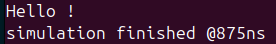
\includegraphics[width=0.8\textwidth]{images/riscv/1-hello_putc.png}
    \caption{Résultat du test \texttt{1-hello\_putc}}
    \label{fig:hello_putc}
\end{figure}

\begin{figure}[htbp]
    \centering
    % width=0.8\textwidth permet de redimensionner l'image à 80% de la largeur de la page
    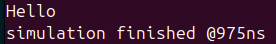
\includegraphics[width=0.8\textwidth]{images/riscv/2-hello_putchar.png}
    \caption{Résultat du test \texttt{2-hello\_putchar}}
    \label{fig:hello_putchar}
\end{figure}

\begin{figure}[htbp]
    \centering
    % width=0.8\textwidth permet de redimensionner l'image à 80% de la largeur de la page
    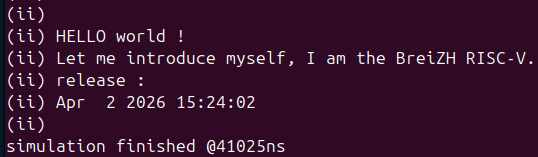
\includegraphics[width=0.8\textwidth]{images/riscv/3-hello_print.png}
    \caption{Résultat du test \texttt{3-hello\_print}}
    \label{fig:hello_print}
\end{figure}

\begin{figure}[htbp]
    \centering
    % width=0.8\textwidth permet de redimensionner l'image à 80% de la largeur de la page
    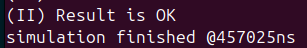
\includegraphics[width=0.8\textwidth]{images/riscv/3-vector-add.png}
    \caption{Résultat du test \texttt{3-vector-add}}
    \label{fig:vector-add}
\end{figure}

\begin{figure}[htbp]
    \centering
    % width=0.8\textwidth permet de redimensionner l'image à 80% de la largeur de la page
    \includegraphics[width=0.8\textwidth]{images/riscv/4-hello\_printf.png}
    \caption{Résultat du test \texttt{4-hello\_printf}}
    \label{fig:hello_printf}
\end{figure}

\begin{figure}[htbp]
    \centering
    % width=0.8\textwidth permet de redimensionner l'image à 80% de la largeur de la page
    \includegraphics[width=0.8\textwidth]{images/riscv/5-riscv\_logo\_uart.png}
    \caption{Résultat du test \texttt{5-riscv\_logo\_uart}}
    \label{fig:riscv_logo_uart}
\end{figure}

\begin{figure}[htbp]
    \centering
    % width=0.8\textwidth permet de redimensionner l'image à 80% de la largeur de la page
    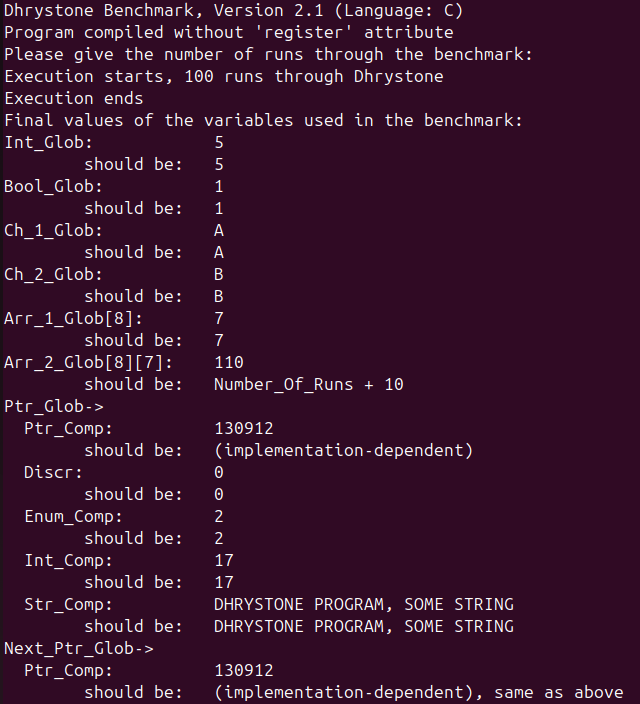
\includegraphics[width=0.8\textwidth]{images/riscv/7-dhrystone0.png}
    \caption{Résultat du test \texttt{7-dhrystone} -- Partie 1}
    \label{fig:dhrystone0}
\end{figure}

\begin{figure}[htbp]
    \centering
    % width=0.8\textwidth permet de redimensionner l'image à 80% de la largeur de la page
    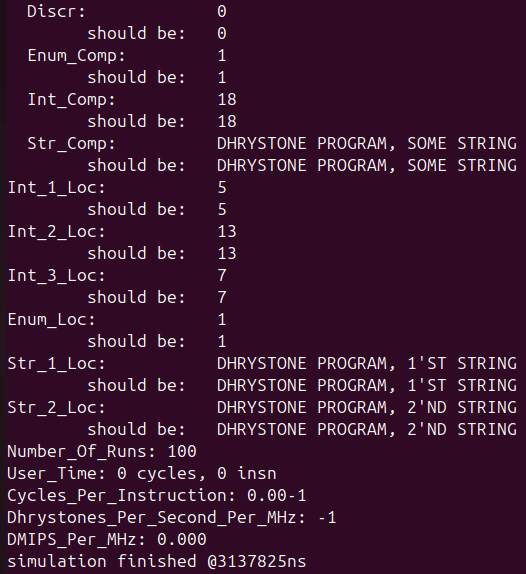
\includegraphics[width=0.8\textwidth]{images/riscv/7-dhrystone1.png}
    \caption{Résultat du test \texttt{7-dhrystone} -- Partie 2}
    \label{fig:dhrystone1}
\end{figure}

\FloatBarrier

\subsection{RISCV\_5STG pipeliné}

Notre cœur RISCV pipeliné fonctionne en simulation seulement sur les premiers tests : \textbf{\texttt{1-hello\_putc}} et \textbf{\texttt{2-hello\_putchar}}.

Il échoue sur les tests  \textbf{\texttt{3-hello\_print}} et \textbf{\texttt{3-vector-add}}. Et ne termine pas comme il faut sur les tests suivants.

Toutefois, on observe tout de même une augmentation des performances de 372\% et 382\% pour les deux premiers tests ce qui est très encourageant pour la suite.

\begin{figure}[htbp]
    \centering
    % width=0.8\textwidth permet de redimensionner l'image à 80% de la largeur de la page
    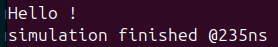
\includegraphics[width=0.8\textwidth]{images/riscv_5stg/1-hello_putc.png}
    \caption{Résultat du test \texttt{1-hello\_putc}}
    \label{fig:hello_putc_5stg}
\end{figure}

\begin{figure}[htbp]
    \centering
    % width=0.8\textwidth permet de redimensionner l'image à 80% de la largeur de la page
    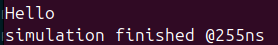
\includegraphics[width=0.8\textwidth]{images/riscv_5stg/2-hello_putchar.png}
    \caption{Résultat du test \texttt{2-hello\_putchar}}
    \label{fig:hello_putchar_5stg}
\end{figure}

\begin{figure}[htbp]
    \centering
    % width=0.8\textwidth permet de redimensionner l'image à 80% de la largeur de la page
    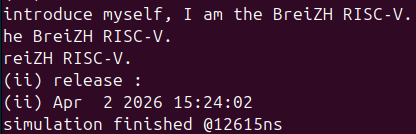
\includegraphics[width=0.8\textwidth]{images/riscv_5stg/3-hello_print.png}
    \caption{Résultat invalide du test \texttt{3-hello\_print}}
    \label{fig:hello_print_5stg}
\end{figure}

\begin{figure}[H]
    \centering
    % width=0.8\textwidth permet de redimensionner l'image à 80% de la largeur de la page
    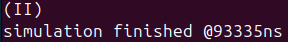
\includegraphics[width=0.8\textwidth]{images/riscv_5stg/3-vector-add.png}
    \caption{Résultat invalide du test \texttt{3-vector-add}}
    \label{fig:vector-add_5stg}
\end{figure}

\end{document}